\documentclass[10pt,twocolumn,twoside]{genpaper}
\usepackage[sort&compress]{natbib}

\usepackage{flushend}
\usepackage{xcolor,colortbl}
\usepackage{subfig}
\usepackage{longtable}
\definecolor{Gray}{gray}{0.9}
\newcommand{\npscarf}{$\mathtt{npScarf}$}
\newcommand{\npscarfg}{$\mathtt{npScarf\_wag}$}
\newcommand{\npreader}{$\mathtt{npReader}$}
\newcommand{\npanalysis}{$\mathtt{npAnalysis}$}
\newcommand{\npbarcode}{$\mathtt{npBarcode}$}
\newcommand{\npgraph}{$\mathtt{npGraph}$}
\newcommand{\canu}{$\mathtt{Canu}$}
\newcommand{\unicycler}{$\mathtt{Unicycler}$}
\newcommand{\spades}{$\mathtt{SPAdes}$}
\newcommand{\albacore}{$\mathtt{Albacore}$}
\newcommand{\racon}{$\mathtt{Racon}$}
\newcommand{\metrichor}{$\mathtt{Metrichor}$}
\newcommand{\minimap}{$\mathtt{minimap2}$}
\newcommand{\miniasm}{$\mathtt{miniasm}$}
\newcommand{\bwa}{$\mathtt{BWA\text{-}MEM}$}

\newcommand{\ec}{\emph{E.~coli}}
\newcommand{\sce}{\emph{S.~cerevisae}}
\newcommand{\kp}{\emph{K.~pneumoniae}} 

\newcommand{\IE}{\emph{i.e.}}
\newcommand{\EG}{\emph{e.g.}}
\newcommand{\review}[1]{\textcolor{red}{#1}}

\title{Online resolving assembly graph by long reads data}
\shorttitle{Real-time Scaffolding with Assembly graph}

%Authors
\author[1]{Son Hoang Nguyen}
\author[1,$\ast$]{Lachlan Coin}

%Affiliation
\affil[1]{Institute for Molecular Bioscience, the University of Queensland, 
St Lucia, Brisbane, QLD 4072 Australia}

\correspondingauthor{
\textsuperscript{$\ast$}
To whom correspondence should be addressed. 
E-mails: author.last@email.com,author.first@email.com
}

%To show compiled date
\compiledate

\begin{document}
%Abstract and keywords have to be defined before \maketitle

\onecolumn
\renewcommand{\figurename}{Supplementary Figure}
\renewcommand{\tablename}{Supplementary Table}
%\setcounter{page}{1}
\setcounter{figure}{0}
\setcounter{table}{0}
% 
\begin{center}
 \Large{Supplementary Information}
\end{center}


\makeatletter

\newlength\oriarrayrulewidth  
\newcount\orilowpenalty
\newcommand\nobreakmidrule{%
 \noalign{\global\oriarrayrulewidth\arrayrulewidth\relax
          \global\orilowpenalty\@lowpenalty\relax  
          \global\@lowpenalty=\numexpr-10000\relax%
          \global\arrayrulewidth\lightrulewidth\relax}
 \hline
 \noalign{\global\@lowpenalty=\orilowpenalty\relax%
          \global\arrayrulewidth\oriarrayrulewidth\relax}}

\makeatother

\begin{longtable}[!hpt]{llcrrrrr}
\caption{Benchmarking \npgraph{} against \npscarf{} versions, $\mathtt{hybridSPAdes}$ and \unicycler{} hybrid assembler with the synthetic data set.}
\label{supp_tab:synthetic_benchmark}\\
\toprule
    &       & Assembly &  & N50  & Mis- &  Mismatch & Indel \\
    & Method & size (bp) & \#Contigs  & (bp) & assemblies & (per $100$Kbp) & (per $100$Kbp) \\
    \hline  
\endfirsthead
\multicolumn{8}{c}%
{\tablename\ \thetable\ -- \textit{Continued from previous page}} \\
\hline
    &       & Assembly &  & N50  & Mis- &  Mismatch & Indel \\
    & Method & size (bp) & \#Contigs  & (bp) & assemblies & (per $100$Kbp) & (per $100$Kbp) \\
\hline
\endhead
\hline \multicolumn{8}{r}{\textit{Continued on next page}} \\
\endfoot
\hline
\endlastfoot

\rowcolor{Gray}
\multicolumn{8}{l}{random sequences no repeats} \\* %
\nobreakmidrule
\rowcolor{Gray}
& npScarf &  4110000 &  3  &  4000000  &  0  & 0.00  & 0.00\\*
\rowcolor{Gray}
& npScarf\_wag & 4109516  &  3  &  4000000  &  0  & 0.00  & 0.00\\*
\rowcolor{Gray}
& npGraph-bwa & 4110000  &  3  &  4000000  &  0  & 0.00  & 0.00\\*
\rowcolor{Gray}
& npGraph-mm2 & 4110000  &  3  &  4000000  &  0  & 0.00  & 0.00\\*
\rowcolor{Gray}
& hybridSPAdes & 4110231  &  3  & 4000077   &  0  & 0.00  &  0.07\\*
\rowcolor{Gray}
& Unicycler & 4110000  &  3  &  4000000  &  0  & 0.00  &  0.00\\
\hline
\multicolumn{8}{l}{random sequences some repeats} \\* %
\nobreakmidrule
& npScarf & 4110940  &  3  &  4002715  &  0  &  0.00 &  0.66\\*
& npScarf\_wag & 4437094  &  7 &  2795129  &  0  &  0.00 &  1.07\\*
& npGraph-bwa & 4110000  &  3  &  4000000  &  0 &  0.00 &  0.00\\*
& npGraph-mm2 &  4110000 &  3  &   4000000 & 0  & 0.00  &  0.00\\*
& hybridSPAdes & 4107566  &  3  &  3999364  &  0  & 0.02  & 0.02\\*
& Unicycler &  4110000 &  3 & 4000000  &  0 & 0.00  &  0.00\\
\hline
\rowcolor{Gray}
\multicolumn{8}{l}{random sequences many repeats} \\* %
\nobreakmidrule
\rowcolor{Gray}
& npScarf &  4316934 &  8  &  3963485  &  24  & 11.55  & 34.54\\*
\rowcolor{Gray}
& npScarf\_wag &  5215965 &  16  &  1515563  &  37  & 0.32  & 7.22\\*
\rowcolor{Gray}
& npGraph-bwa & 4110000  &  3  &  4000000  &  0  &  0.32 & 0.15\\*
\rowcolor{Gray}
& npGraph-mm2 &  4110000 &  3  &  4000000  &  0  & 0.32  & 0.15\\*
\rowcolor{Gray}
& hybridSPAdes & 4108190  &  3  &  3999621  &  0  &  0.68 &  0.15\\*
\rowcolor{Gray}
& Unicycler & 4110000  &  3  &  4000000  &  0  &  0.32  & 0.15  \\
\hline
% \pagebreak
% \toprule
\multicolumn{8}{l}{\emph{Acinetobacter} A1} \\* %
\nobreakmidrule
& npScarf & 3912299  &  3  &  3870269  &  4  & 4.74  & 13.02 \\*
& npScarf\_wag & 3945166  &  3  &  3906368  &  1  & 7.00  & 14.02 \\*
& npGraph-bwa & 3918374  &  2  &  3909643  &  0 & 16.34  & 0.61 \\*
& npGraph-mm2 & 3885898  &  2  &  3877167  & 1 & 18.05  & 1.03 \\*
& hybridSPAdes &  3929948 &  53  &  3353679  &  0  & 35.48  & 3.22\\*
& Unicycler & 3917745  &  2 & 3909014  & 0  & 2.50  &  0.13\\
\hline
\rowcolor{Gray}
\multicolumn{8}{l}{\emph{Acinetobacter} AB30} \\* %
\nobreakmidrule
\rowcolor{Gray}
& npScarf & 4512464  &  7  &  4304628  &  35  & 57.95  & 72.87\\*
\rowcolor{Gray}
& npScarf\_wag & 5315235  &  13  &  1267710  &  136  &  73.55 & 8.15\\*
\rowcolor{Gray}
& npGraph-bwa & 4335342  &  2  &  4148952  &  1  & 16.93  & 1.45\\*
\rowcolor{Gray}
& npGraph-mm2 & 4335790  &  1  &  4335790  & 0   &  6.97 & 0.25\\*
\rowcolor{Gray}
& hybridSPAdes & 4337369  &  3  &  2701005  &  0  &  12.80 &  1.39\\*
\rowcolor{Gray}
& Unicycler &  4333041 &  1  &  4333041  &  1  &  6.42 &  0.53\\
\hline
\multicolumn{8}{l}{\ec{} K12 MG1655} \\* %
\nobreakmidrule
& npScarf & 4649902  &  2  &  4641702  &  4  & 14.94  & 34.35 \\*
& npScarf\_wag &  4687952 &  3  &  4641732  &  0  & 6.55  &  1.96\\*
& npGraph-bwa & 4641743  &  1  &  4641743  & 0  &  4.50 & 0.43 \\*
& npGraph-mm2 & 4641820  &  1  &  4641820  &  0 &  3.88 & 0.26 \\*
& hybridSPAdes &  4644555 &  1  &  4641036  &  0  & 0.62  & 0.09\\*
& Unicycler & 4641650  &  1 &  4641650 &  0 & 3.43  & 0.26 \\
\hline
\rowcolor{Gray}
\multicolumn{8}{l}{\ec{} O25b H4-ST131} \\* %
\nobreakmidrule
\rowcolor{Gray}
& npScarf &  5245913 &  3  &  5095571  &  7  &  7.05 & 18.81\\*
\rowcolor{Gray}
& npScarf\_wag & 5292700  &  3  &  3469617  &  9  &  9.03 & 1.55\\*
\rowcolor{Gray}
& npGraph-bwa & 5237821  &  7  &  4049493  &  1  &  3.38 & 0.31\\*
\rowcolor{Gray}
& npGraph-mm2 &  5249799 &  3  &  5110117  &  0  &  2.40 & 0.15\\*
\rowcolor{Gray}
& hybridSPAdes & 5252762  &  8  &  4258948  &  2  &  5.43 &  0.57\\*
\rowcolor{Gray}
& Unicycler & 5249442  &  3  &  5109760  &  0  & 4.02 & 0.27 \\
\hline
% \pagebreak
% \toprule
\multicolumn{8}{l}{\emph{Klebsiella} 30660 NJST258 1} \\* %
\nobreakmidrule
& npScarf & 5559772  &  7  &  5259053  &  4  & 17.18  & 13.48\\*
& npScarf\_wag & 5613780  &  7  &  5268535  &  6  & 1.59  & 1.92\\*
& npGraph-bwa & 5534843  &  8  &  5263229  &  0  & 3.15  & 0.76\\*
& npGraph-mm2 & 5534878  &  8  &  5263264  &  0  & 2.75  & 0.74\\*
& hybridSPAdes &  5545668 & 8   &  5545668  &  2  & 4.95  & 0.09 \\*
& Unicycler & 5537860  &  9  &  5263196  &  0  & 1.34  & 0.51 \\
\hline
\rowcolor{Gray}
\multicolumn{8}{l}{\emph{Klebsiella} MGH 78578} \\* %
\nobreakmidrule
\rowcolor{Gray}
& npScarf &  5729304 &  5  &  5316429  &  12  & 14.90  & 20.27\\*
\rowcolor{Gray}
& npScarf\_wag & 5754443  &  5  &  3026286  &  16  &  8.17 & 2.56\\*
\rowcolor{Gray}
& npGraph-bwa &  5695801 &  7  &  5311745  &  1  & 12.65  & 1.25\\*
\rowcolor{Gray}
& npGraph-mm2 & 5696302  &  6  &  5315267  &  0  &  6.06 & 0.44\\*
\rowcolor{Gray}
& hybridSPAdes &  5706470 &  11  &  5315273  &  1  & 3.82  &  0.67\\*
\rowcolor{Gray}
& Unicycler &  5694231 &  14  &  5315096  &  0  & 5.38 &  0.21\\
\hline
\multicolumn{8}{l}{\emph{Klebsiella} NTUH-K2044} \\* %
\nobreakmidrule
& npScarf & 5471696  &  2  &  5249198  &  6  & 4.82  &  8.55\\*
& npScarf\_wag & 5530559  &  3  &  5249369  &  2  &  2.25 &  1.35\\*
& npGraph-bwa & 5472629  &  2  &  5248476  & 0  & 2.52  &  0.31\\*
& npGraph-mm2 &  5472655 &  2  &  5248503  &  0 &  1.21 &  0.26\\*
& hybridSPAdes & 5473572  &  2  &  5248894  &  0  &  0.44 & 0.15\\*
& Unicycler & 5472697  & 2  & 5248545  &  0 & 2.41  &  0.35\\
\hline
\rowcolor{Gray}
\multicolumn{8}{l}{\emph{Mycobacterium tuberculosis} H37Rv} \\* %
\nobreakmidrule
\rowcolor{Gray}
& npScarf &  4498245 &  4  & 4402238   &  8  & 5.15  & 2.68\\*
\rowcolor{Gray}
& npScarf\_wag &  4506056 &  4  &  4410942  &  3  & 6.81  & 2.59\\*
\rowcolor{Gray}
& npGraph-bwa & 4411406  &  1  &  4411406  &  0  & 1.88  & 0.43\\*
\rowcolor{Gray}
& npGraph-mm2 & 4411532  & 1   &  4411532  &  0  & 0.68  & 0.00\\*
\rowcolor{Gray}
& hybridSPAdes & 4413942  &  1  &  4410519  &  0  &  0.75 &  0.11\\*
\rowcolor{Gray}
& Unicycler & 4411538  &  1  &  4411538  &  0  &  2.22 &  0.34\\
\hline
% \pagebreak
% \toprule
\multicolumn{8}{l}{\emph{Saccharomyces cerevisiae} S288c} \\* %
\nobreakmidrule
& npScarf &  11986800 &  24  &  796769  &  51  &  62.12 & 21.46 \\*
& npScarf\_wag & 12003203  &  21  &  917017  &  21  & 69.14  & 5.47 \\*
& npGraph-bwa & 11921736  &  40  &  913090  &  3 &  38.04 &  1.94\\*
& npGraph-mm2 & 11920984  &  38  &  913198  &  2 &  20.66 &  0.95\\*
& hybridSPAdes &  12027533 &  45  &  770543  &  5  & 32.58  & 1.94\\*
& Unicycler &  11847655 & 72  & 909114  &  0 & 21.81  &  1.04\\
\hline
\rowcolor{Gray}
\multicolumn{8}{l}{\emph{Shigella dysenteriae}  Sd197} \\* %
\nobreakmidrule
\rowcolor{Gray}
& npScarf &  4586075 &  173  & 36560   &  55  & 120.14  & 111.59\\*
\rowcolor{Gray}
& npScarf\_wag & 5462918  &  92  &  98791  &  105  &  147.48 & 79.28\\*
\rowcolor{Gray}
& npGraph-bwa & 4564058  &  6  &  4369264  &  5  & 80.64  & 11.16\\*
\rowcolor{Gray}
& npGraph-mm2 & 4558920  &  6  &  4364264  &  7  & 75.51  & 10.98\\*
\rowcolor{Gray}
& hybridSPAdes &  4519131 & 23   &  821249  & 96   & 9.57  &  1.42\\*
\rowcolor{Gray}
& Unicycler & 4560901  & 3   &  4369231  &  0  & 11.88  & 1.05 \\
\hline
\multicolumn{8}{l}{\emph{Shigella sonnei} 53G} \\* %
\nobreakmidrule
& npScarf &  6441461 &  20  &  1953896  &  82  & 164.02  &  219.52\\*
& npScarf\_wag & -  &  -  &  -  &  -  & -  &  -\\*
& npGraph-bwa & 5211544  &   4 &  4988532  & 0  & 14.53  &  0.31\\*
& npGraph-mm2 & 5211527  &  4  &   4988519 & 0  &  8.56 &  0.17\\*
& hybridSPAdes & 5223875  &  8  &  2195455  &  2  & 41.92  & 0.06\\*
& Unicycler &  5220517 &  5 &  4988548 & 0  & 7.39  &  0.52\\
\hline
\rowcolor{Gray}
\multicolumn{8}{l}{\emph{Streptococcus suis} BM407} \\* %
\nobreakmidrule
\rowcolor{Gray}
& npScarf &  2183951 & 3   &  2146594  &  0  & 21.51  & 9.17\\*
\rowcolor{Gray}
& npScarf\_wag & 2289880  &  3  &  1493189  &  1  & 3.17  & 1.96\\*
\rowcolor{Gray}
& npGraph-bwa & 2154623  &  6  &  2131479  &  1  & 5.25  & 0.28\\*
\rowcolor{Gray}
& npGraph-mm2 & 2149876  &  6  &  2146774  &  0  & 1.44  & 0.28\\*
\rowcolor{Gray}
& hybridSPAdes & 2172703  &  2  &  2146237  &  0  & 6.82  &  0.09\\*
\rowcolor{Gray}
& Unicycler &  2170829 &   2 &  2146250  &  0  &  2.67 & 0.32 \\
\hline
\end{longtable}

\begin{figure}[!hpt]
\centering
\subfloat[\emph{Citrobacter~freundii} CAV1374]{
	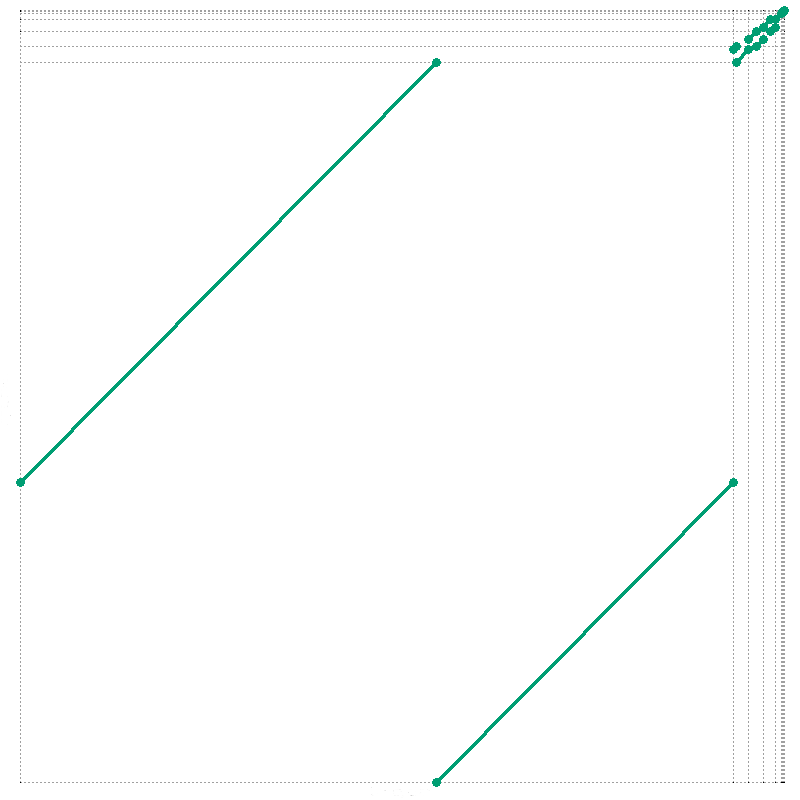
\includegraphics[width=.45\textwidth]{images/dp_c_freundii_cav1374.png}
}
\hfill
\subfloat[\emph{Klebsieall~oxytoca} CAV1015]{
	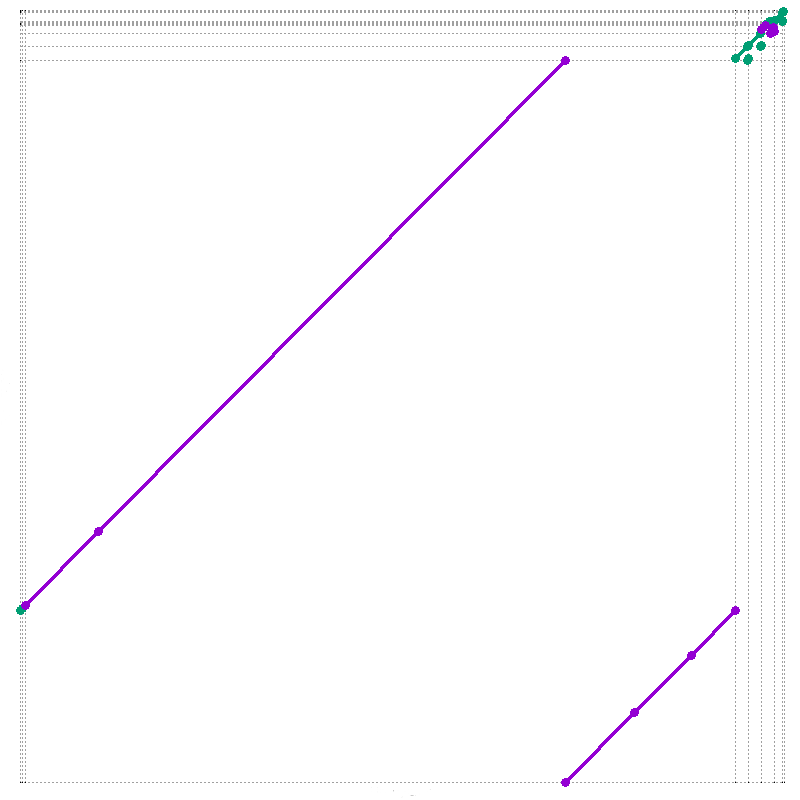
\includegraphics[width=.45\textwidth]{images/dp_k_oxytoca_cav1015.png}
}
\\
\subfloat[\emph{Enterobacter~cloacae} CAV1411]{
	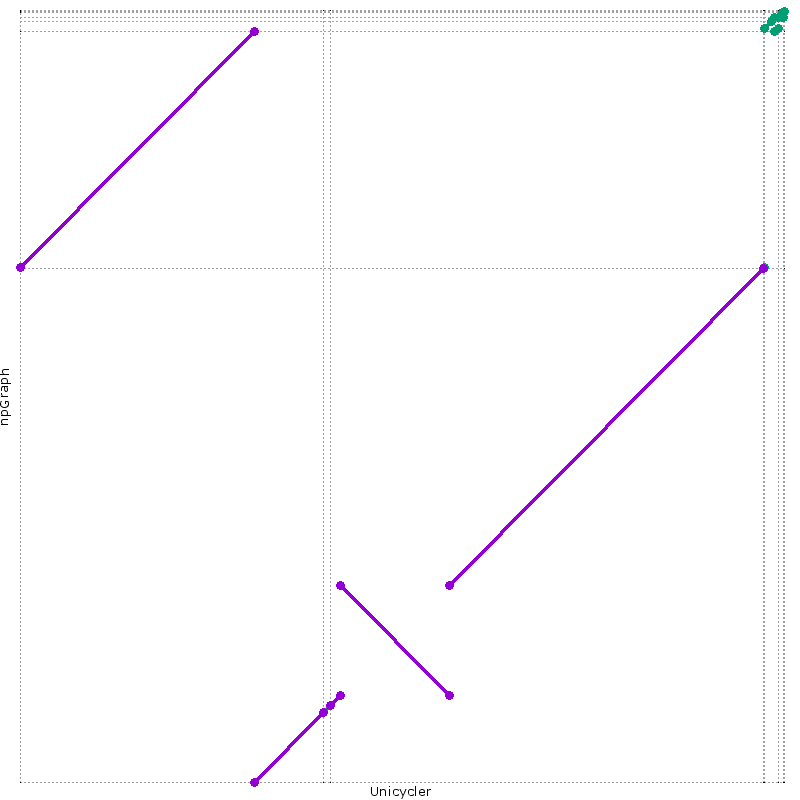
\includegraphics[width=.45\textwidth]{images/dp_e_cloacae_cav1411.png}
}
\caption[Dotplot generated by MUMmer for assembly results of \unicycler{} versus \npgraph{}.]{Dotplot generated by MUMmer for assembly results of \unicycler{} versus \npgraph{}. Structural agreements between two methods were found in (a)~\emph{C.freundii} and (b)~\emph{K.oxytoca} assembly contigs. On the other hand, for (c)~\emph{E.cloacae} sample, there was a disagreement detected between 2 largest contigs given by two assembly algorithms. This case is investigated more thoroughly by using a reference from a same bacterial strain in Figure~\ref{supp_fig:npgraph_ref}.}
\label{supp_fig:npgraph_dotplot}
\end{figure}

\begin{figure}[!hpt]
\centering
\subfloat[\emph{E.~cloacae} \unicycler{} assembly versus reference genome]{
	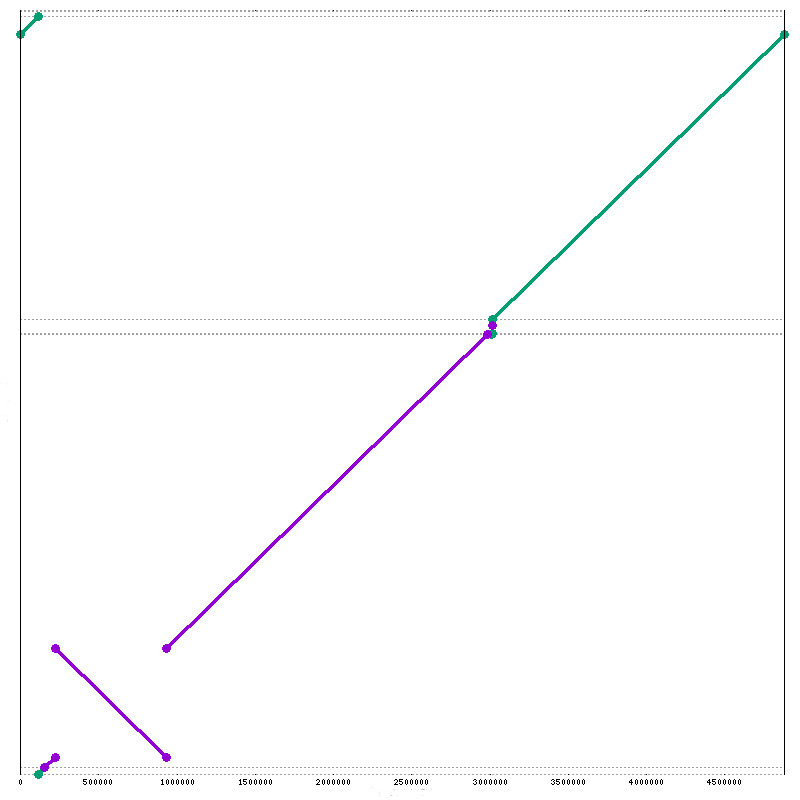
\includegraphics[width=.5\textwidth]{images/dp_ref_unicycler.png}
}
\hfill
\subfloat[\emph{E.~cloacae} \npgraph{} assembly versus reference genome]{
	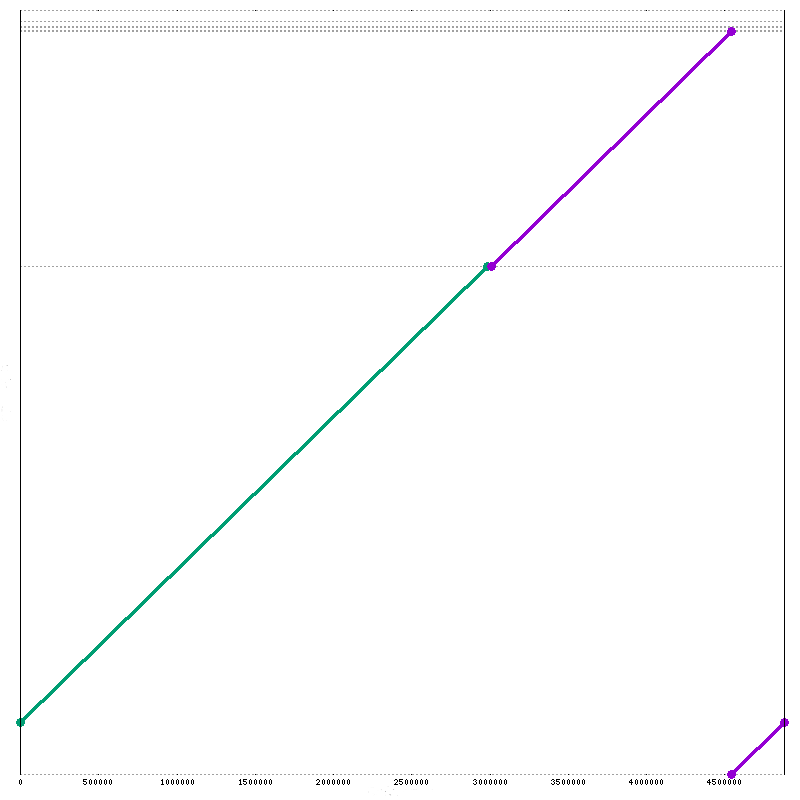
\includegraphics[width=.5\textwidth]{images/dp_ref_npgraph.png}
}
\caption[Alignments of a \emph{Enterobacter~cloacae} reference genome to assembly sequences generated by \unicycler{} and \npgraph{}]{Alignments of an \emph{Enterobacter~cloacae} reference genome to assembly sequences generated by  (a)~\unicycler{} and (b)~\npgraph{}. While the former presents a structural variant, the latter is virtually an 1-to-1 mapping.}
\label{supp_fig:npgraph_ref}
\end{figure}

\end{document}
